\section{Validation}\label{sec:valid}
\paragraph{Internal consistency.} The integrated density reproduces the number of valence electrons (e.g.\ $\int\rho\,dV=40.000$ for SrTiO$_3$ from SIESTA). A \code{.den\_fmt}$\to$CHGCAR$\to$read round trip changes the density by $\sim10^{-8}$, and the CHGCAR files written by the JavaScript and Python implementations differ by $\sim10^{-6}$ (relative), at the level of the printed precision. After each extension of the input layer, all CASTEP outputs of a reference calculation were compared byte by byte with those of the previous version. The density-difference report, the comparison table and the effective masses give the same numbers in the browser and on the command line.

\paragraph{Reference systems.} Table~\ref{tab:valid} lists results obtained with real output files distributed with the test suites of pymatgen (VASP), sisl (SIESTA), Quantum ESPRESSO and cclib (ORCA). The PBE band gap of Si (0.614\,eV, indirect from $\Gamma$ to near X) and the longitudinal electron mass ($m^*_l=0.94\,m_e$, experiment $0.92\,m_e$) agree with the literature for this functional; the ferromagnetic Fe$_2$O$_3$ cell computed with LDA+U carries 20\,$\mu_\mathrm B$ (56 spin-up and 36 spin-down electrons), as expected for four high-spin Fe$^{3+}$ ions; the SrTiO$_3$ LDA calculation shows an indirect R$\to\Gamma$ gap of 2.25\,eV with O~2p valence and crystal-field-split Ti~3d $t_{2g}/e_g$ conduction states, and the integrated density matches the 40 valence electrons. In every case the analysis reproduces the physical picture expected for these well-studied systems. The band-gap correction illustrates the limits of empirical models: for Si the PBE$\to G_0W_0$ relation predicts 1.738\,eV against the experimental 1.17\,eV, an error within the scatter of the original fit but large in absolute terms for small-gap semiconductors; the scissor to the experimental value restores 1.170\,eV exactly, with identical effective masses, as expected for a rigid shift. The browser and command-line implementations give identical corrected gaps.

\begin{table}[t]\centering\small
\caption{Validation with real outputs. Gaps are Kohn–Sham gaps of the functional used in each calculation.}\label{tab:valid}
\begin{tabularx}{\linewidth}{@{}llX@{}}\toprule
Code & System & \BMR\ result \\\midrule
CASTEP & MgH$_2$:Fe (162-atom supercell, spin) & $\eF=1.837$\,eV; total gap 1.394\,eV, indirect M$\to$R; Fe–H 1.649–1.653\,\AA \\
VASP & Si, line-mode bands (PBE) & gap 0.614\,eV indirect; $m^*_e=0.94\,m_e$; $m^*_h(\Gamma)=0.32\,m_e$ \\
VASP & Si, gap correction (Section~\ref{sec:gapcorr}) & empirical model 1.738\,eV; scissor to experiment 1.170\,eV; masses unchanged \\
VASP & Fe$_2$O$_3$, ferromagnetic (LDA+U) & 56$\uparrow$/36$\downarrow$ electrons, 20\,$\mu_\mathrm B$; $P(\eF)$ undefined ($\eF$ in gap) \\
SIESTA & SrTiO$_3$, spin-polarised (LDA) & gap 2.25\,eV indirect R$\to\Gamma$; $t_{2g}$ below $e_g$; $\int\rho\,dV=40.000$\,e \\
SIESTA & Bi$_2$Se$_3$ (no spin--orbit) & gap 0.042\,eV, direct; eigenvalues identical to sisl \\
QE & Si, test-suite reference (2 $\bm{k}$-points) & gap 1.32\,eV on the coarse mesh \\
ORCA & divinylbenzene (molecule) & HOMO–LUMO gap 5.18\,eV; Mulliken and Löwdin charges \\\bottomrule
\end{tabularx}
\end{table}

\paragraph{Cross-validation against established tools.} Table~\ref{tab:bench} compares \BMR\ with pymatgen, sumo, sisl, cclib and pybader on the same output files (script \code{tools/comparar\_ferramentas.py}). Gaps, band edges, Fermi energies, spin-resolved electron counts and molecular-orbital energies agree to the printed precision ($|\Delta|\le10^{-4}$\,eV). Two differences are methodological and favour the approach adopted here. (i) For MgH$_2$:Fe, the highest occupied band exceeds the Fermi energy written by CASTEP by only 0.04--0.17\,meV (an offset far below any physical energy scale, presumably because the Fermi level is determined on the self-consistent mesh rather than on the band-path $\bm k$-points); tools based on pymatgen therefore classify the system as metallic and report a zero gap, whereas electron counting yields 1.394\,eV, identical (to $10^{-4}$\,eV) to the value obtained by applying the same criterion to the eigenvalues parsed by sumo. (ii) For Si, the conduction-band minimum lies between two $\mathbf{k}$-points of the path; a parabola anchored at the sampled $\mathbf{k}$-point yields one-sided masses of 0.68 and 1.54\,$m_e$ (sumo), whereas the fit with a linear term used by \BMR\ locates the true minimum and gives 0.94\,$m_e$, close to the experimental 0.92\,$m_e$. For the 162-atom MgH$_2$:Fe density, the refined Bader charges agree with pybader within $8\times10^{-4}$\,e per atom on average (0.026\,e at most), with identical total charge, compared with 0.013\,e for the on-grid assignment alone; the refined partition took 0.7\,s, against 1.2\,s for pybader. The Brillouin zones of the six recognised lattice types reproduce $V_\mathrm{BZ}=(2\pi)^3/V$ to $10^{-6}$ and, for FCC Si, the exact distances $|X|=2\pi/a$, $|L|=\sqrt3\pi/a$, $|W|=\sqrt5\pi/a$ and $|K|=3\sqrt2\pi/2a$. The space groups of all 51 library materials and of seven reference structures read from symmetrised CIF and POSCAR files are recovered in both implementations, with identical high-symmetry points in the browser and on the command line; for the MgH$_2$:Fe supercell, moyo finds the base-centred orthorhombic group $Cmmm$ produced by the defect and the relaxation, and the corresponding ORCC path is used. For 18 reference structures covering all 14 Bravais lattices and 23 of the 25 Setyawan--Curtarolo cases (the remaining MCLC4 is a measure-zero boundary case), every high-symmetry point lies on the zone surface, the moduli $|\bm k|$ agree with the independent implementation in pymatgen \cite{ong2013pymatgen} to $10^{-8}$\,\AA$^{-1}$ (triclinic lattices, whose reduced basis is not unique, and the boundary case ORCF3 excepted), and the browser and Python give identical points. This check also exposed that the point $F_3$ listed for MCLC1 in the original paper does not lie on the zone surface; it is not part of the path and is omitted, as in pymatgen.
\begin{table}[t]\centering\small
\caption{Cross-validation of \BMR\ against established tools on the same output files. $|\Delta|$ is the absolute difference.}\label{tab:bench}
\resizebox{\linewidth}{!}{\begin{tabular}{@{}lllrrlr@{}}\toprule
Code & System & Quantity & \BMR & Reference & Tool & $|\Delta|$ \\\midrule
VASP & Si (PBE) & gap (eV) & 0.6143 & 0.6143 & pymatgen & 1.1e-16 \\
VASP & Si (PBE) & $E_\mathrm{F}$ (eV) & 5.8561 & 5.8561 & pymatgen & 1.3e-05 \\
VASP & Si (PBE) & CBM$-$VBM (eV) & 0.6143 & 0.6143 & pymatgen & 1.1e-16 \\
VASP & Si (PBE) & $m^*_e$, side 1 ($m_e$) & 0.9410 & 0.6771 & sumo & 2.6e-01 \\
VASP & Si (PBE) & $m^*_e$, side 2 ($m_e$) & 0.9410 & 1.5400 & sumo & 6.0e-01 \\
VASP & Si (PBE) & $m^*_e$ vs experiment ($m_e$) & 0.9410 & 0.9200 & experiment & 2.1e-02 \\
VASP & Fe$_2$O$_3$ (LDA+U) & moment ($\mu_\mathrm{B}$) & 20.0000 & 20.0000 & pymatgen & 1.6e-06 \\
VASP & Fe$_2$O$_3$ (LDA+U) & gap $\uparrow$ (eV) & 4.0199 & 4.0199 & pymatgen & 0.0e+00 \\
VASP & Fe$_2$O$_3$ (LDA+U) & gap $\downarrow$ (eV) & 2.1923 & 2.1923 & pymatgen & 0.0e+00 \\
CASTEP & MgH$_2$:Fe (162 at.) & total gap (eV) & 1.3940 & 0.0000 & sumo & 1.4e+00 \\
CASTEP & MgH$_2$:Fe (162 at.) & $E_\mathrm{F}$ (eV) & 1.8368 & 1.8368 & sumo & 4.2e-06 \\
CASTEP & MgH$_2$:Fe (162 at.) & gap, electron counting on sumo eigenvalues (eV) & 1.3940 & 1.3941 & sumo & 7.4e-05 \\
SIESTA & SrTiO$_3$ (LDA) & total gap (eV) & 2.2500 & 2.2500 & sisl & 0.0e+00 \\
SIESTA & Bi$_2$Se$_3$ & gap (eV) & 0.0418 & 0.0418 & sisl & 6.0e-16 \\
ORCA & divinylbenzene & HOMO (eV) & -4.0652 & -4.0652 & cclib & 1.8e-05 \\
ORCA & divinylbenzene & LUMO (eV) & 1.1197 & 1.1197 & cclib & 5.9e-06 \\
ORCA & divinylbenzene & HOMO--LUMO gap (eV) & 5.1849 & 5.1849 & cclib & 1.2e-05 \\
CHGCAR & MgH$_2$:Fe CHGCAR (162 at.) & Bader (on-grid) mean $|\Delta q|$ (e) & 0.0000 & 0.0127 & pybader & 1.3e-02 \\
CHGCAR & MgH$_2$:Fe CHGCAR (162 at.) & Bader (refined) mean $|\Delta q|$ (e) & 0.0000 & 0.0008 & pybader & 8.0e-04 \\
CHGCAR & MgH$_2$:Fe CHGCAR (162 at.) & Bader $\sum q$ (e) & 651.0000 & 651.0000 & pybader & 2.3e-13 \\
CHGCAR & MgH$_2$:Fe CHGCAR (162 at.) & Bader (refined) max.\ $|\Delta q|$ (e) & 0.0000 & 0.0257 & pybader & 2.6e-02 \\
\bottomrule\end{tabular}}
\end{table}



\begin{figure}[t]\centering
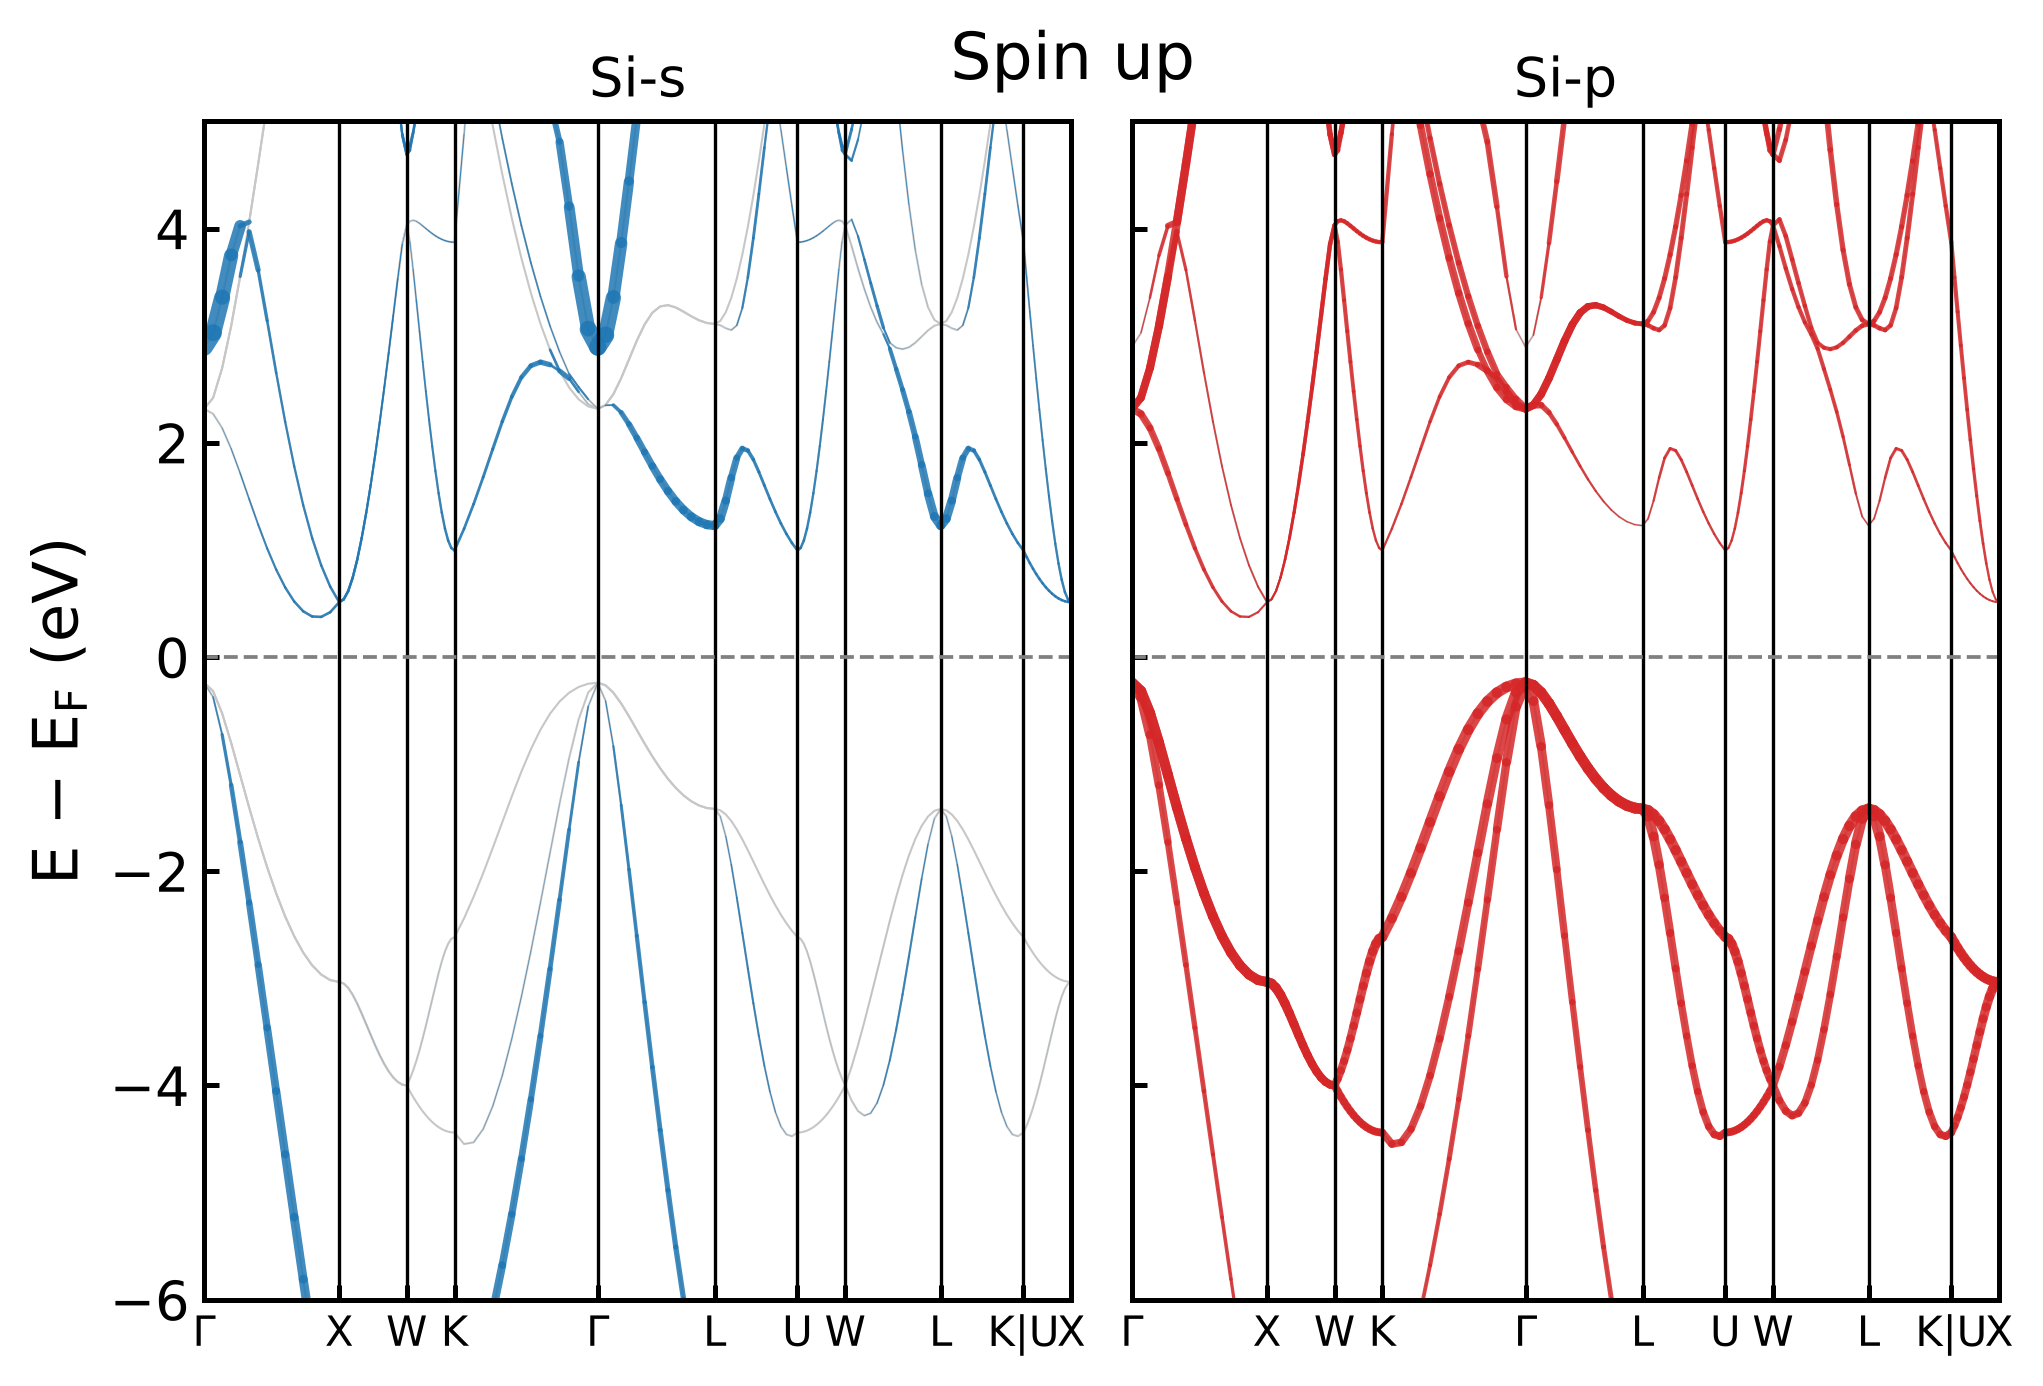
\includegraphics[width=0.49\linewidth]{figures/si_fat.png}\hfill
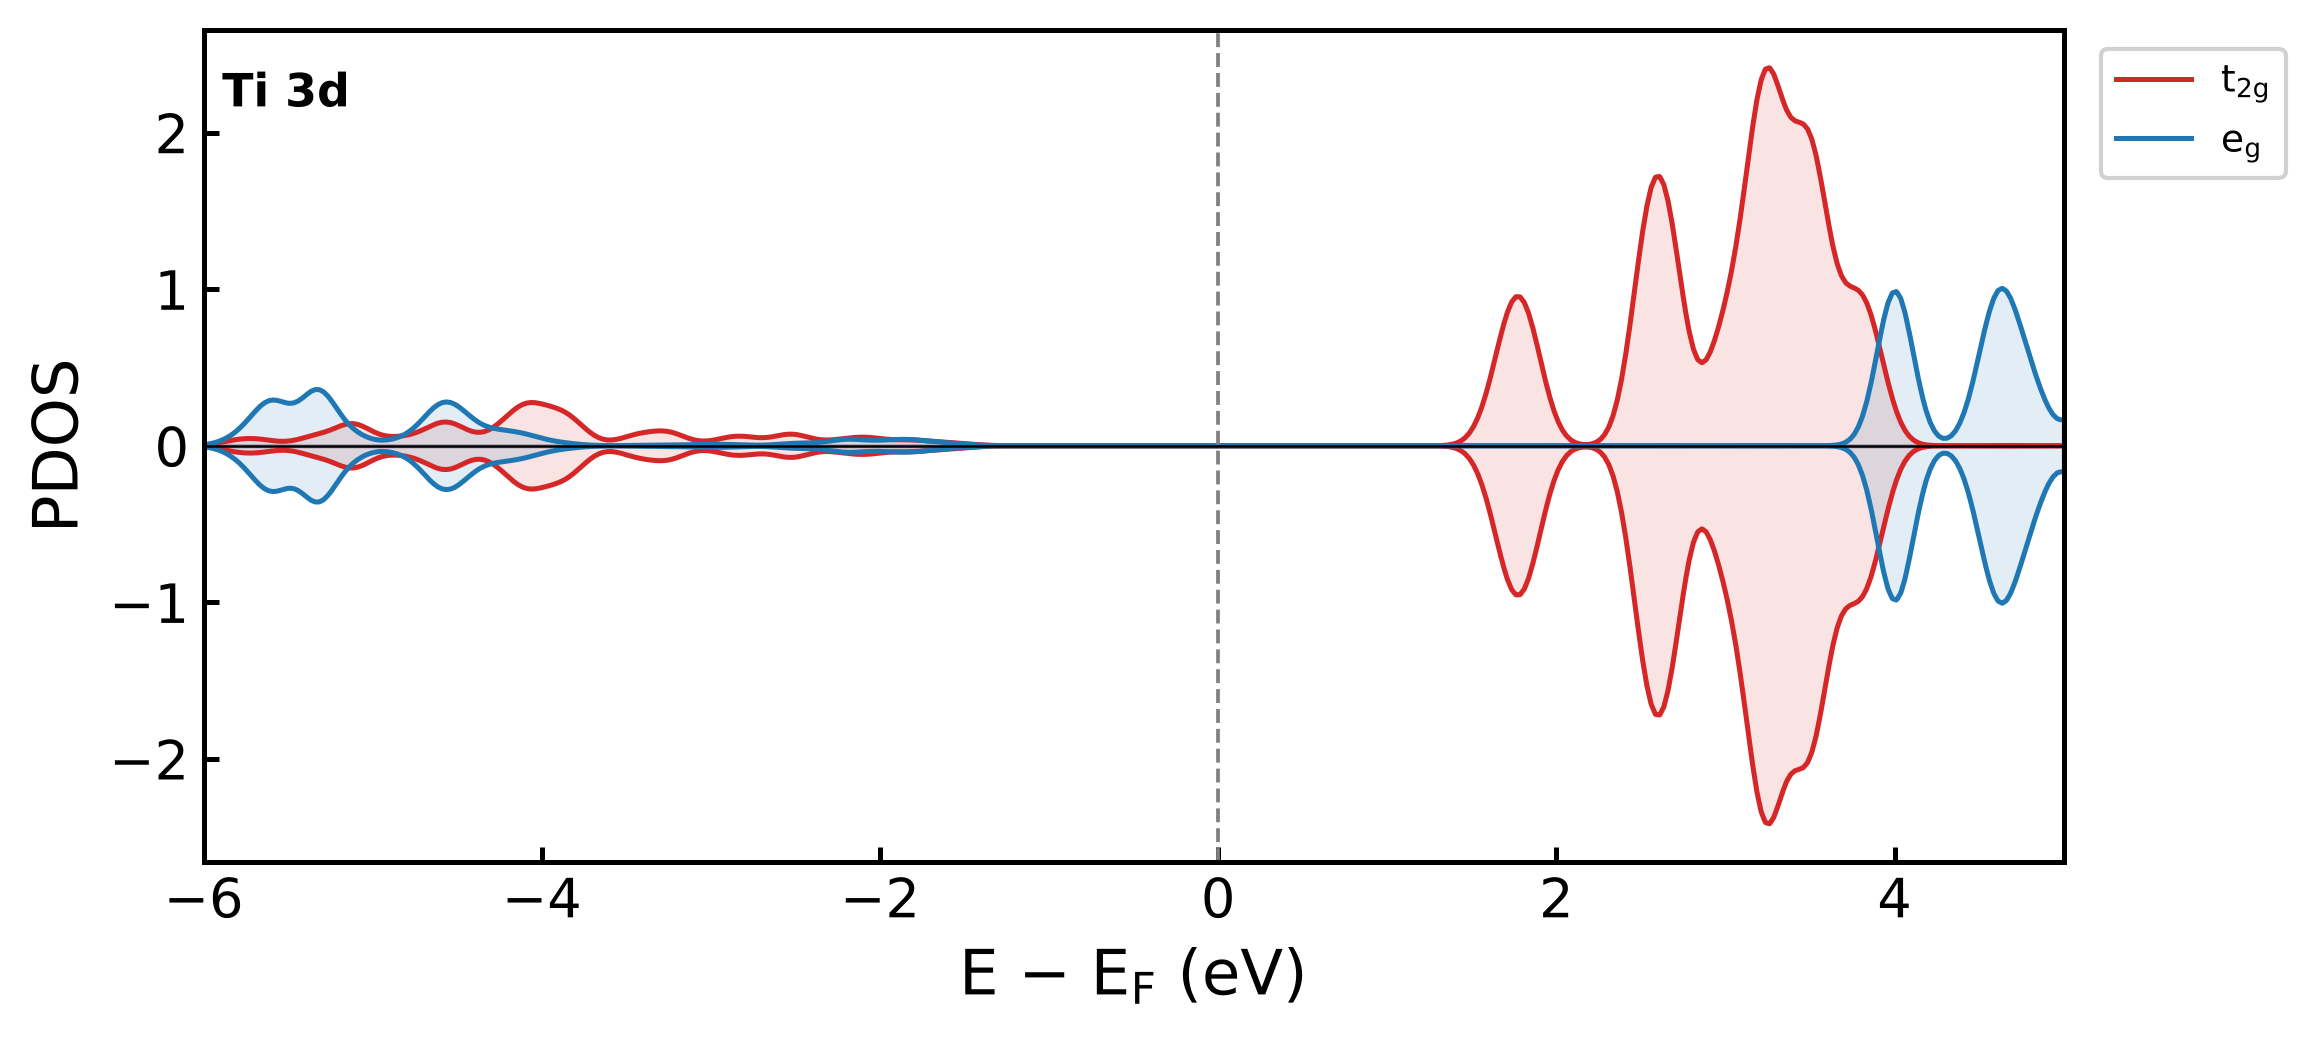
\includegraphics[width=0.49\linewidth]{figures/sto_t2g.png}
\caption{Left: projected bands of Si (VASP): $s$ character at the bottom of the valence band and $p$ character at its top. Right: Ti~3d PDOS of SrTiO$_3$ (SIESTA) split into $t_{2g}$ and $e_g$ by the octahedral crystal field.}\label{fig:valid}
\end{figure}
